\section{How to build an \ab{} workflow system}

\begin{frame}{What is \express{}, though?}
    A Julia-written
    \begin{itemize}
        \item extensible,
        \item lightweight,
        \item high-throughput,
        \item high-level
    \end{itemize}
    workflow framework that aims to automate \ab{} calculations for the materials science
    community.
\end{frame}

\begin{frame}{What is needed in an \ab{} workflow system?}
    There are at least three components:

    \begin{itemize}
        \item Sciency, technical stuff: calculations, input generation, output analysis...
        \item Dispatcher, job scheduler: interacting with \ab{} software, \texttt{mpi}...
        \item User interface: interacting with users
    \end{itemize}
\end{frame}

\section{How to build an \ab{} workflow system}

\subsection{Sciency, technical stuff}

\subsubsection{Binary dependencies \& foreign function interface}

\begin{frame}
    \frametitle{\subsubsecname}
    \framesubtitle{Building an artifact}

    Operations like finding the symmetry of a crystal
    are very common in \ab{} calculations (usually the first step).
    Therefore, we need a good library to do this.

    There is a C library called \href{https://github.com/spglib/spglib}{\texttt{spglib}}
    that does this.
    To make it a productive library, we need first put it in a container
    (``artifacts''). Luckily, the amazing Julia community has made it possible:
    \href{https://github.com/JuliaBinaryWrappers/spglib_jll.jl}{\texttt{spglib_jll.jl}}.
\end{frame}

\begin{frame}[fragile]
    \frametitle{\subsubsecname}
    \framesubtitle{Foreign function interface}

    \begin{columns}
        \begin{column}{0.3\textwidth}
            Now that we have an artifact that exports the functions of the C library,
            it may still be hard to use since it uses some C data structures and API, which may
            not be idiomatic in Julia. Therefore, we need to wrap it with a higher level of APIs.
            \href{https://github.com/singularitti/Spglib.jl}{\texttt{Spglib.jl}} is built based on
            this expectation.
        \end{column}

        \begin{column}{0.7\textwidth}
            {\tiny
                \begin{algorithmblock}
                    \begin{juliaverbatim}
function standardize_cell(
    cell::Cell;  # `Cell` was not defined in the C library
    to_primitive = false,
    no_idealize = false,
    symprec = 1e-5,
)
    @unpack lattice, positions, types = _expand_cell(cell)
    to_primitive = Base.cconvert(Cint, to_primitive)
    no_idealize = Base.cconvert(Cint, no_idealize)
    num_atom = Base.cconvert(Cint, length(types))
    allocations = 4
    _positions = Matrix{Cdouble}(undef, 3, num_atom * allocations)
    _types = Vector{Cint}(undef, num_atom * allocations)
    _positions[:, 1:num_atom] = positions
    _types[1:num_atom] = types
    n = ccall(
        (:spg_standardize_cell, libsymspg),
        Cint,
        (Ptr{Cdouble}, Ptr{Cdouble}, Ptr{Cint}, Cint, Cint, Cint, Cdouble),
        lattice,
        _positions,
        _types,
        num_atom,
        to_primitive,
        no_idealize,
        symprec,
    )
    return Cell(transpose(lattice), _positions[:, 1:n], _types[1:n])
end
                    \end{juliaverbatim}
                \end{algorithmblock}
            }
        \end{column}
    \end{columns}
\end{frame}

\subsubsection{Parsers for \ab{} software I/O}

\begin{frame}[allowframebreaks]{\subsubsecname}
    Most \ab{} software is written in Fortran and has plain text files as input \& output.
    Therefore, we need parsers for both of them. But it is tricky...

        {\footnotesize
            \begin{itemize}
                \item For example, \qe{}'s input adopts the \texttt{Namelist} data structure from
                      Fortran. Julia does not have a parser for Fortran...
                \item A Python package
                      (\href{https://github.com/marshallward/f90nml}{\texttt{f90nml}}) can do that.
                      I wrote a very preliminary package
                      \href{https://github.com/singularitti/PyFortran90Namelists.jl}{\texttt{PyFortran90Namelists.jl}},
                      to call that Python code.
                \item However, it uses \texttt{PyCall.jl}, so sometimes people have trouble installing
                      it if they already have Python installed
                      (see \href{https://github.com/JuliaPy/PyCall.jl\#specifying-the-python-version}{``Specifying the Python version''}).
            \end{itemize}
        }

    For output files, it is even more complicated since they usually do not have a standard
    format. Therefore lots of regular expressions need to be used.
    It is extremely error-prone. I used
    \href{https://github.com/jkrumbiegel/ReadableRegex.jl}{\texttt{ReadableRegex.jl}} to build them.
\end{frame}

\subsubsection{A wrapper for \ab{} software executables}

\begin{frame}[fragile, allowframebreaks]{\subsubsecname}
    To run external \ab{} software within Julia, what should we do?\\

    Use the Julia \texttt{AbstractCmd}s? Good choice!
    But sometimes, we want to generate a series of \texttt{AbstractCmd}s dynamically,
    especially in a workflow system.
    Writing them one by one is not so efficient.\\

    Wait, can we write functions to generate \texttt{AbstractCmd}s? Then all the command
    arguments will be standard Julia function arguments! For example,

    {\scriptsize
            \begin{algorithmblock}
                \begin{juliaverbatim}
mpirun -np 16 pw.x -npool 2 -nk 2 -input scf_in > scf_out
                \end{juliaverbatim}
            \end{algorithmblock}
        }

    will be

        {\scriptsize
            \begin{algorithmblock}
                \begin{juliaverbatim}
pw("scf_in", "scf_out"; np = 16, npool = 2, nk = 2)
                \end{juliaverbatim}
            \end{algorithmblock}
        }

    \framebreak

    What's more, we could use
    \href{https://github.com/comonicon/Comonicon.jl}{\texttt{Comonicon.jl}},
    to build new executables that will provide customized arguments
    (see \href{https://github.com/MineralsCloud/QuantumESPRESSOCommands.jl}{\texttt{QuantumESPRESSOCommands.jl}})

    {\scriptsize
            \begin{algorithmblock}
                \begin{juliaverbatim}
using Comonicon: @cast
@cast function pw(input, output = mktemp(parentdir(input))[1];
                  np = 1, npool = 1, nk = 1, path = "pw.x", chdir = false)
    ...
    return run(cmd)
end
                \end{juliaverbatim}
            \end{algorithmblock}
        }

    Therefore, we could run it with

        {\scriptsize
            \begin{algorithmblock}
                \begin{juliaverbatim}
pw -np 16 -npool 2 -nk 2 -input scf_in scf_out
            \end{juliaverbatim}
            \end{algorithmblock}
        }

\end{frame}


\subsection{Dispatcher and job scheduler}

\begin{frame}{\subsecname}
    The core of \express{} is its dispatching system,
    which is implemented by
    \href{https://github.com/MineralsCloud/SimpleWorkflows.jl}{\texttt{SimpleWorkflows.jl}},
    taking inspiration from
    \href{https://github.com/invenia/Dispatcher.jl}{\texttt{Dispatcher.jl}}
    (currently unmaintained) and
    \href{https://github.com/cihga39871/JobSchedulers.jl}{\texttt{JobSchedulers.jl}}.

    \begin{columns}[t]
        \begin{column}{0.4\textwidth}
            \begin{center}
                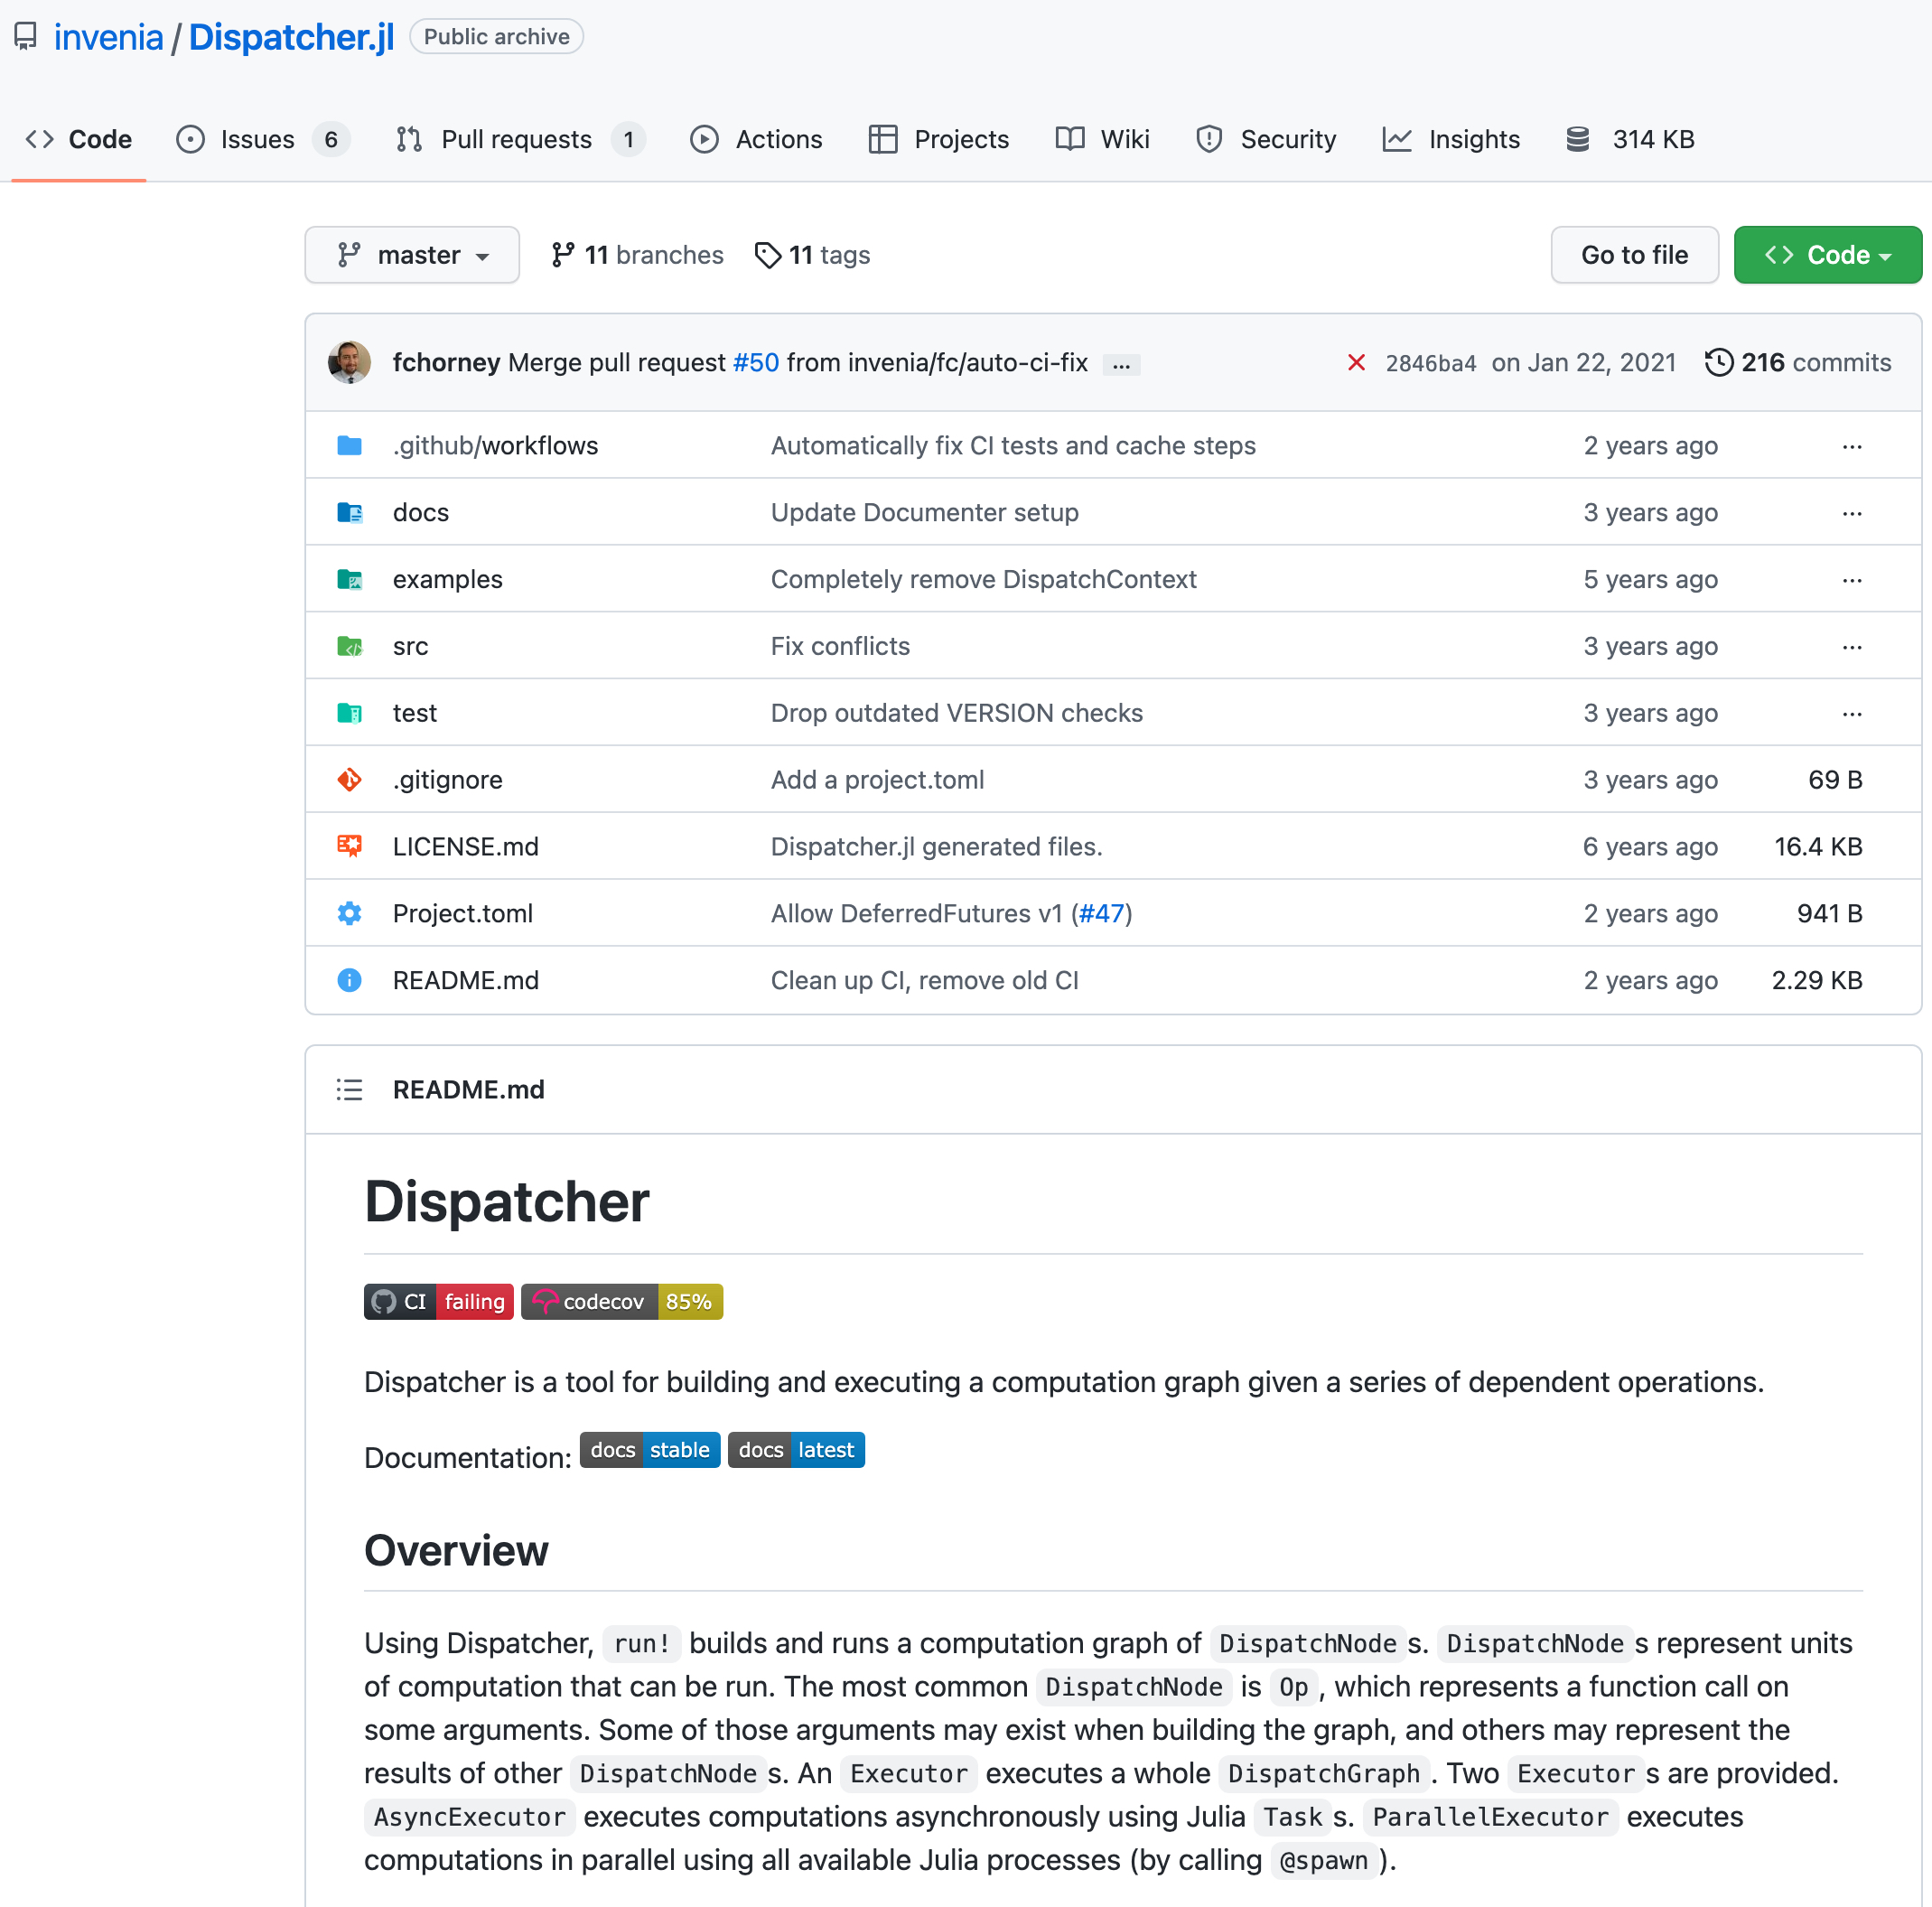
\includegraphics[height=0.5\textheight]{Dispatcher}
            \end{center}
        \end{column}
        \hfill
        \begin{column}{0.4\textwidth}
            \begin{center}
                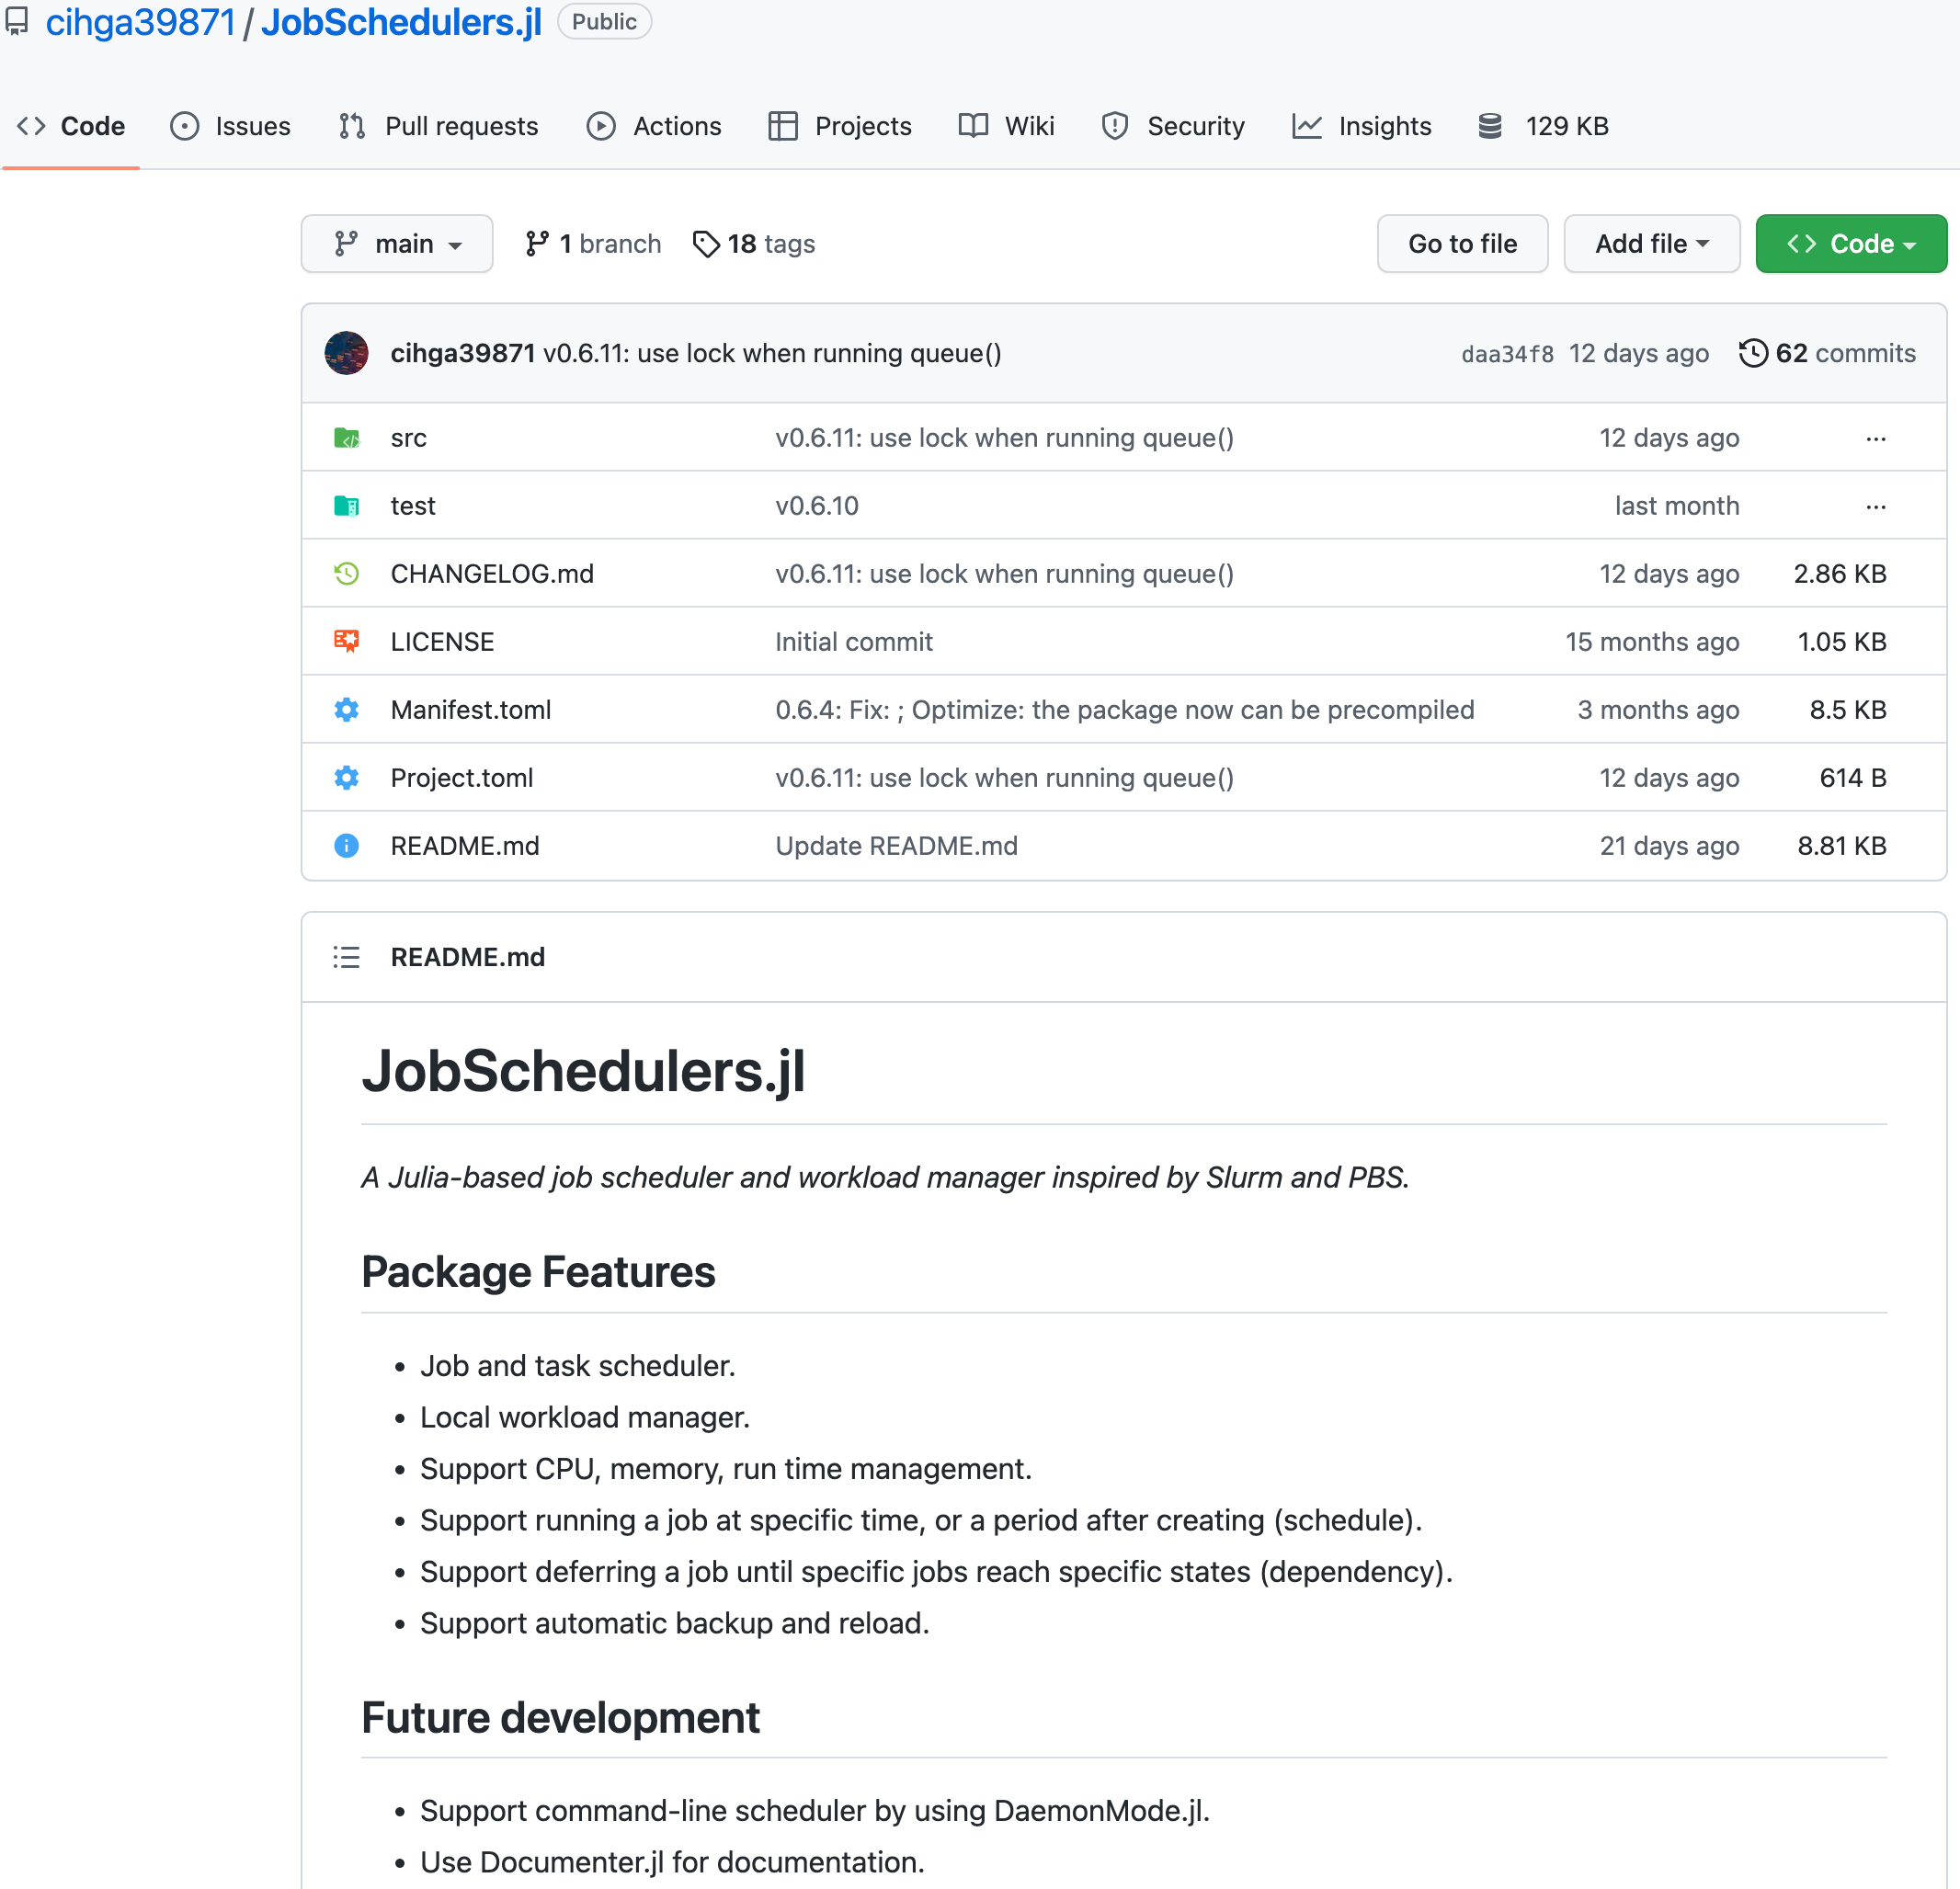
\includegraphics[height=0.5\textheight]{JobSchedulers}
            \end{center}
        \end{column}
    \end{columns}
\end{frame}

\begin{frame}[fragile]
    \frametitle{\subsecname}
    \framesubtitle{Design overview}

    The simplest atomic operation in a \texttt{Workflow} is called a \texttt{Job}.
    It tracks the time, result, and other info of the user's input.
    The relationship between each \texttt{Job} in the \texttt{Workflow} is represented by a
    DAG.\\

    To construct a \texttt{Workflow}, we provide some operators to simplify this step.

        {\footnotesize
            \begin{algorithmblock}
                \begin{juliaverbatim}
using SimpleWorkflows: →, ⇉, ⇶, ↣

a0 → a ⇉ b ⇶ c ↣ d0 → d → f → g ⇉ h ⇶ i ↣ j0 → j → l
        \end{juliaverbatim}
            \end{algorithmblock}
        }
\end{frame}

% [fragile] needed when the content contains juliaverbatim.
\begin{frame}[fragile, allowframebreaks]
    \frametitle{\subsecname}
    \framesubtitle{An example}

    Let's construct an arbitrary \texttt{Workflow}:
    {\scriptsize
    \begin{algorithmblock}
        \begin{juliaverbatim}
using SimpleWorkflows
i = @job (println("Start job `i`!"); sleep(5)) user = "me" desc = "i"
j = @job (println("Start job `j`!"); sleep(3); exp(2)) user = "me" desc = "j"
k = @job (println("Start job `k`!"); sleep(6)) desc = "k"
l = @job (println("Start job `l`!"); run(`sleep 3`)) desc = "l" user = "me"
m = @job (println("Start job `m`!"); sleep(3); sin(1)) desc = "m"
n = @job (println("Start job `n`!"); run(`pwd` & `ls`)) user = "me" desc = "n"
i → l
j → k → m → n
j → l
k → n
wf = Workflow(k)
        \end{juliaverbatim}
    \end{algorithmblock}
    }

    \framebreak

    The DAG of the \texttt{Job}s from \texttt{i} to \texttt{n} is

    \begin{figure}[H]
        \centering
        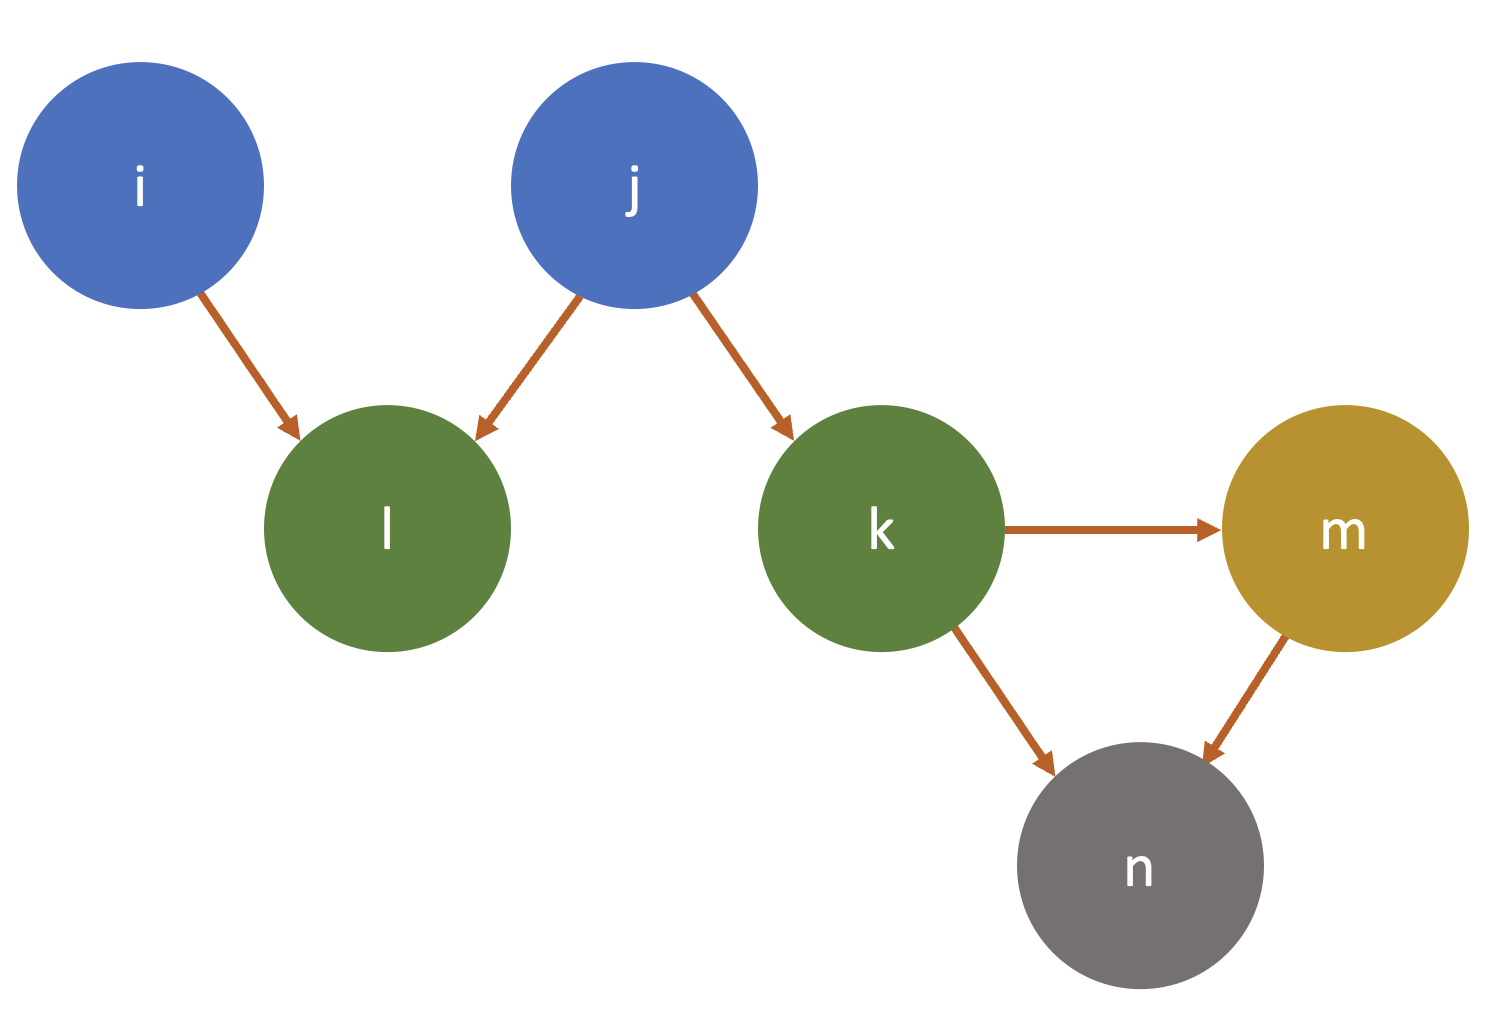
\includegraphics[height=0.35\textheight]{order}
        \caption{The execution order of the \texttt{Job}s from \texttt{i} to \texttt{n}.
            Blue circles are the first, then green, then yellow, and gray is the last.}
        \label{fig:order}
    \end{figure}

    \texttt{Jobs} of the same order are executed in parallel or asynchronously by
    Kahn's algorithm.

    \framebreak

    After or during the execution of the \texttt{Workflow}, we can use \texttt{queue} to
    print all the \texttt{Job}s' information:

    {\scriptsize
    \begin{algorithmblock}
        \begin{juliaverbatim}
run!(wf)
queue()
        \end{juliaverbatim}
    \end{algorithmblock}
    }

    \begin{figure}[H]
        \centering
        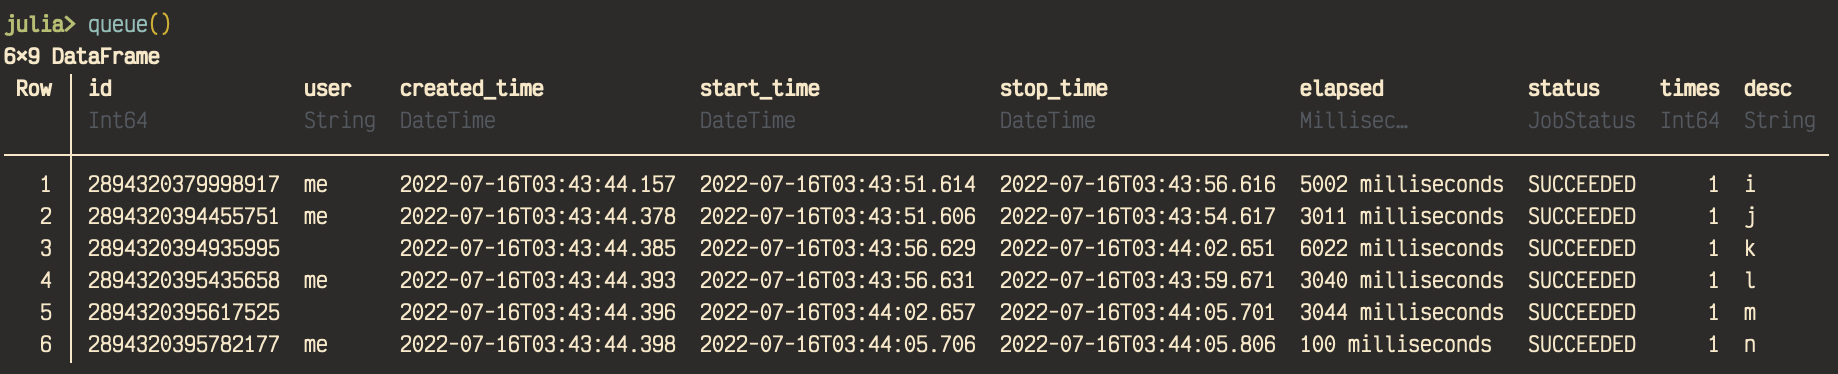
\includegraphics[width=0.8\textwidth]{queue}
        \caption{Queuing the information of the \texttt{Job}s in a \texttt{Workflow}.}
        \label{fig:queue}
    \end{figure}

    And a \texttt{JLD2} format file will be saved during this step. If some errors happen
    during the running or the execution is interrupted, we can rerun only the
    failed/interrupted \texttt{Jobs} according to the information saved in that file.
\end{frame}

\subsection{User interface}\label{ssec:ui}

\begin{frame}
    \frametitle{\subsecname}
    \framesubtitle{Motivation}

    \begin{block}{What should be the most commonly-used interface}
        Since most tasks in different \ab{} calculations are routine, with only
        input parameters changed. It is desirable to make an interface that takes a few
        parameters each time.

        A command line interface plus a template file for the \ab{} software for the sciency
        fixed settings and a configuration file for the computational variables is a
        balanced choice.
    \end{block}

    \begin{block}{Command line interface}
        We want a command line interface to have

        \begin{itemize}
            \item A single topmost command (\texttt{xps})
            \item A few second-tier commands corresponding to different workflows
            \item A few third-tier commands corresponding to different tasks in a workflow
            \item A few arguments, flags, and options for each command mentioned above
        \end{itemize}
    \end{block}
\end{frame}

% [fragile] needed when the content contains juliaverbatim.
\begin{frame}[fragile, allowframebreaks]
    \frametitle{\subsecname}
    \framesubtitle{Implementation}

    With \href{https://github.com/comonicon/Comonicon.jl}{\texttt{Comonicon.jl}}, we can implement
    an aforementioned interface easily.

        {\scriptsize
            \begin{algorithmblock}
                \begin{juliaverbatim}
module ExpressCommands
using Comonicon: @cast, @main

@cast function print(file)
    ...
end

@main
end
                \end{juliaverbatim}
            \end{algorithmblock}
        }

    Then we can run

        {\scriptsize
            \begin{algorithmblock}
                xps print config.toml
            \end{algorithmblock}
        }

    to print a configuration file, for example.

    \framebreak

    To build subcommands for different workflows, we use modules inside the global module
    (\texttt{ExpressCommands}) to do that:

    {\scriptsize
    \begin{algorithmblock}
        \begin{juliaverbatim}
module ExpressCommands

module EOS

using Comonicon: @cast

@cast function fit(calc, cfgfile)
    ...
end

end

end
        \end{juliaverbatim}
    \end{algorithmblock}
    }

    See package \texttt{ExpressCommands.jl} for more details.
\end{frame}

\begin{frame}
    \frametitle{\subsecname}
    \framesubtitle{Run commands with configuration files}

    \begin{columns}[t]
        \begin{column}{0.4\textwidth}
            As stated in previous slides, we could put computational settings
            in a configuration file to change variables dynamically.

            We make use of
            \href{https://github.com/Roger-luo/Configurations.jl}{\texttt{Configurations.jl}},
            which can read TOML files into a Julia \texttt{struct}
            (similar to \href{https://github.com/quinnj/JSON3.jl}{\texttt{JSON3.jl}}).
            We accept JSON and YAML formats as well.

            A typical configuration file looks like this (items may change in the future versions):
        \end{column}

        \begin{column}{0.6\textwidth}
            \begin{minted}[frame=single, linenos]{toml}
            recipe = "eos"
            template = "template.in"
            [cli.mpi]
            np = 128
            [save]
            status = "status.jls"
            eos = "eos.jls"
            [trial_eos]
            type = "bm3"
            values = ["300.44 bohr^3", "74.88 GPa", 4.82]
            [fixed.pressures]
            unit = "GPa"
            values = [-5, -2, 0, 5, 10, 15, 17, 20]
        \end{minted}
        \end{column}
    \end{columns}

\end{frame}


